  %%%%%%%%%%%%%%%%%%%%%%%%%%%%%%%%%%%%%%% -*- coding: utf-8; mode: latex -*- %%
  %
%%%%%                       CHAPTER
 %%%
  %

\chapter{Results and discussion}
%\addcontentsline{lof}{chapter}{\thechapter\quad Nihil Molestiae}
%\addcontentsline{lot}{chapter}{\thechapter\quad Nihil Molestiae}
\label{ch:omnisvoluptas}

%\begin{quotation}
%  {\small\it Neque porro quisquam est qui dolorem ipsum quia dolor sit amet, consectetur, adipisci velit...}

%{\small\it -- Cerico}
%\end{quotation}


\section{Classification Experiments}

For this work, three types of experiments have been conducted, each using two different architectures, as described in the previous chapter. Results are shown in tables \textbf{5.1} and \textbf{5.2} (for the baseline experiments), \textbf{5.3} and \textbf{5.4} (for the semi-independent experiments), and \textbf{5.1} and \textbf{5.6} (for the language independent experiments). These tables show the top five MLP parameter configurations for each of the experiments. Tables \textbf{5.1}, \textbf{5.3} and \textbf{5.5} present the results for architecture 1, whereas tables \textbf{5.2}, \textbf{5.4} and \textbf{5.6} communicate the results for architecture 2.

\subsection{Baseline experiments}

Tables \textbf{5.1} and \textbf{5.2} show that both architecture 1 and 2 of the \gls{mlp} yielded an accuracy of 90\% with the best parameterization. \\
All the best models configurations (for both architecture 1 and 2) achieved higher scores using the GITA dataset. There are multiple reasons that can justify this result. For example, the audios from the MDVR\_KCL dataset were recorded using phone calls, which uses audio compression with losses, resulting in audios with inferior quality. The distribution between \gls{mlp} solvers (adam and lbfgs) on the top 5 model configurations for architecture 1 is well balanced, whereas 4 out of the 5 (or 80\%) of the best model configurations on architecture 2 use the adam solver. From the three values used for the alpha parameter, the Both architectures have yielded better results when using valuer smaller values (0.0001 and 0.001) for the alpha parameter, comparing to the results obtained using larger values (0.1). Finally, architecture 1 doesn't show significant differences between models using 2000 and 5000 for the maximum number of iterations. On the other hand, this difference is observable on architecture 2, where the 4 models which yielded better results use the value of 5000 for this parameter. The difference between architectures be explained by the extra complexity of architecture 2 derived from the large number of parameters to optimize (52400 weights and 401 biases), compared with architecture 1, which has 3844 weights and 63 bias. The large number of parameter requires a larger number of iterations for the model to converge.
Architecture 1 yielded precision values between 0.75 and 1, meaning that 75\% to 100\% of the patients labeled as \gls{pd} by the models were correctly classified. Architecture 2 produced slightly worst results regarding precision, achieving values between 67\% and 100\%. Recall values (which evaluates how the percentage of \gls{pd} patients were correctly classified) were similar between the two architectures. Architecture 1 produced recall values between 71\% and 100\%, whereas architecture 2 achieved results between 67\% and 100\%. Using the specificity metric (which allows to evaluate the percentage of \gls{hc} patients that were correctly classified) to compare the two architectures, architecture 2 outperformed architecture 1 by a small margin, producing a range of values between 75\% and 100\%, whereas architecture 1 produced a range of values between 80\% and 100\%. Finally, comparing both architectures using the F1-score metric, it is possible to see a significantly higher performance with architecture 2, which produced a maximum of almost 91\%, compared with architecture 1 that returned a maximum of 85\%.
We can conclude that there are no significant differences between the two architectures. \\
 - Compare with state-of-the-art (compare with the ones using the same dataset and use that as an argument)
 
\begin{table}
	\centering
	\begin{tabular}{lcccccccc}
		\bfseries dataset & \bfseries solver & \bfseries alpha & \bfseries iterations & \bfseries accuracy  & \bfseries precision & \bfseries recall & \bfseries specificity & \bfseries f1-score
		\csvreader[head to column names]{csvs/baseline_top.csv}{}
		{\\\hline\dataset & \solver & \alpha & \iterations & \accuracy  & \precision & \recall & \specificity & \fscore}
	\end{tabular}
	\caption{\label{tab:table-name}Baseline experiment results using architecture 1.}
\end{table}

\begin{table}
	\centering
	\begin{tabular}{lcccccccc}
		\bfseries dataset & \bfseries solver & \bfseries alpha & \bfseries iterations & \bfseries accuracy  & \bfseries precision & \bfseries recall & \bfseries specificity & \bfseries f1-score
		\csvreader[head to column names]{csvs/baseline_200_top.csv}{}
		{\\\hline\dataset & \solver & \alpha & \iterations & \accuracy  & \precision & \recall & \specificity & \fscore}
	\end{tabular}
	\caption{\label{tab:table-name}Baseline experiment result using architecture 2.}
\end{table}

\subsection{Semi-independent experiments}

As observed in \textbf{table 5.3}, when testing a semi-independent approach, architecture 1 yielded higher results than architecture 2. Despite the two best model configurations of both architectures produced an accuracy of 90\%, the following 3 model configurations resulted in an accuracy of almost 86\%, whereas architecture 2 only reached an accuracy of 80\%.  \\
Architecture 1 produced its best results using a combination of FraLusoPark and Gita datasets. At the same time, higher scores from architecture 2 were achieved when combining Gita and MDVR\_KCL. Similarly to the baseline experiments, it is possible to observe that the models produce better results when trained with the Gita dataset. No differences can be observed between results achieved with the different values for the solver parameter (adam and lbfgs), nor for the number of maximum iterations. On the other hand, 4 out of the top 5 results for architecture 1 and all the top 5 results for architecture 2 are produced using smaller values of the alpha parameter (0.0001 and 0.001). This results are similar to what was observed in the baseline experiments.
Architecture 1 outperformed architecture 2 on precision, producing results between 0.83 and 1, whereas architecture 2 yielded values between 0.6 and 1. While both architectures' higher value was the same, architecture 1 produced consistently more consistent results, with a smaller. Similar results were achieved when using recall. Architecture 1 produced values between 0.75 and 1, and 3 of the top 5 model configurations achieved 100\% recall. On the other hand, architecture 2 values for recall ranged from 0.66 and 1. As F1-score combines the values from precision and recall (and architecture 1 outperformed architecture 2 on both these metrics), the same results were achieved with the F1-score metric. Values of this metric for architecture 1 varied between 0.85 and 0.92, whereas architecture 2 values ranged from 0.75 to 0.88. Finally, architecture 2 produced better results when using specificity. This architecture's values varied between 0.71 and 1, with a much smaller variation between extremes when compared to the results produced by architecture 1, which varied from 0.5 to 1.
The results were similar to the ones achieved on the baseline experiences using architecture 2. Architecture 1 had a slightly better performance on the semi language-independent experiments, compared to the baselines.
This experiment, coupling with similar work that tested semi language-independent models \textbf{citar o gajo que fez semi-independent}, allows to conclude that a model can be retrained with a small dataset of a new language and extended to be used with a new language with the same performance as it was trained only with the new language. This can be particularly beneficial for this problem, as lack of training data is usually a limitation to train such models.

\begin{table}
	\centering
	\begin{tabular}{lcccccccc}
		\bfseries dataset & \bfseries solver & \bfseries alpha & \bfseries iterations & \bfseries accuracy  & \bfseries precision & \bfseries recall & \bfseries specificity & \bfseries f1-score
		\csvreader[head to column names]{csvs/semi_top.csv}{}
		{\\\hline\dataset & \solver & \alpha & \iterations & \accuracy  & \precision & \recall & \specificity & \fscore}
	\end{tabular}
	\caption{\label{tab:table-name}Semi-independent experiment result using architecture 1.}
\end{table}

\begin{table}
	\centering
	\begin{tabular}{lcccccccc}
		\bfseries dataset & \bfseries solver & \bfseries alpha & \bfseries iterations & \bfseries accuracy  & \bfseries precision & \bfseries recall & \bfseries specificity & \bfseries f1-score
		\csvreader[head to column names]{csvs/semi_200_top.csv}{}
		{\\\hline\dataset & \solver & \alpha & \iterations & \accuracy  & \precision & \recall & \specificity & \fscore}
	\end{tabular}
	\caption{\label{tab:table-name}Semi independent experiment result using architecture 2.}
\end{table}

\subsection{Language-independent experiments}
 - Com o modelo 100\% independente obtivemos XXX de performance \\
When using a language-independent model, architecture 1 achieved a maximum accuracy of 67\%. Architecture 2 yelded very similar results, scoring a maximum of 66\%. \\
 - A performance atingida não foi semelhante à do estado da arte \\
 - Comparar os parametros \\
 Combining the top 5 model configurations for both architectures, almost all of these (90\%) obtained its score when trained with the FraLusoPark and MDVR\_KCL, and tested with Gita. The same percentage of the combination of the top 5 models of each architecture used the lbfgs solver, whereas only 1 of these 10 model configurations used the adam solver. Similarly to what was observed on the dependent and semi-independent experiments, the model's performance is constantly higher when smaller values are used for the alpha parameter. On both architectures, only 1 of the top 5 model configurations used $\alpha = 1$. Finally, no significant differences can be found when comparing model's performance based on the number of iterations. \\
 - Avaliar as outras métricas \\
Considering the precision metric, architecture 1 scored higher values than architecture 2. It's values range between 0.59 and 0.64 whereas architecture 2 yielded values between 0.57 and 0.61, meaning that architecture 2 produced more false positives (patients from the \gls{hc} group wrongly classified as \gls{pd}). On the other hand, architecture 1 performed worse when comparing the recall metric, only achieving values ranging from 0.76 to 0.84, whereas architecture 2 scored recall values between 0.77 and 0.88, thus correctly classifying a higher number of patients from the \gls{pd} group. Architecture 1 significantly outperformed architecture 2, when compared using the specificity metric. Architecture 2 only achieved a maximum of 0.46, compared to architecture 1, which scored a maximum of 0.58 on this metric. Lastly, as F1-score combines precision and recall in the same metric, the results of both architectures on this metric were equivalent.
- Avaliar correlação dos parametros da rede com os resultados
Figures \textbf{1} and \textbf{2} compare the different values of each parameter of the \gls{mlp} with the accuracy yielded by the model.

 - Overall, o modelo X/Y apresentou uma performance superior ao outro \\

 - Overall de quantos doentes fomos capazes de dignosticar \\

\begin{table}
	\centering
	\begin{tabular}{lcccccccc}
		\bfseries dataset & \bfseries solver & \bfseries alpha & \bfseries iterations & \bfseries accuracy  & \bfseries precision & \bfseries recall & \bfseries specificity & \bfseries f1-score
		\csvreader[head to column names]{csvs/independent_top.csv}{}
		{\\\hline\dataset & \solver & \alpha & \iterations & \accuracy  & \precision & \recall & \specificity & \fscore}
	\end{tabular}
	\caption{\label{tab:table-name}Independent experiment result using architecture 1.}
\end{table}

\begin{table}
	\centering
	\begin{tabular}{lcccccccc}
		\bfseries dataset & \bfseries solver & \bfseries alpha & \bfseries iterations & \bfseries accuracy  & \bfseries precision & \bfseries recall & \bfseries specificity & \bfseries f1-score
		\csvreader[head to column names]{csvs/independent_200_top.csv}{}
		{\\\hline\dataset & \solver & \alpha & \iterations & \accuracy  & \precision & \recall & \specificity & \fscore}
	\end{tabular}
	\caption{\label{tab:table-name}Independent experiment result using architecture 2.}
\end{table}

\subsection{Model optimization}

When comparing models' results per parameter, it is possible to find the best values for each. Smaller values for alpha (0.0001 and 0.001) consistently produced superior results when compared with 0.01. Considering language dependent and semi language dependent models, there is no evident difference between the use of the lbfgs and adam solvers. For both experiments,  around 50\% of the model configurations used each solver. On the other hand, for language-independent experiments, it is clear that models using the lbfgs solver outperformed those using the adam solver. As we can see in tables \textbf{5.5} and \textbf{5.6}, between the top 5 model configurations of each architecture, only 1 was trained using adam. Lastly, comparing the results based on the number of maximum number of iterations ($\#interations$), there is no evident difference between models trained with $\#iterations = 2000$ and $\#iterations = 5000$ in any of the experiments performed. This shows that, in most cases, 2000 iterations should be sufficient to train the model, and convergence is achieved without executing the maximum number of iterations.

\section{Language Independency}

Both architectures used during this work yielded an accuracy of 90\% on the semi language-independent experiments. This results are inferior to the ones achieved on a similar work (\cite{parkinson_three_languages}), where the authors were able to achieve a maximum accuracy of 96\% when training a model with a German dataset and 80\% of a Spanish dataset and testing with the remaining 20\%. On the other hand, this model was outperformed by Architecture 1 when using the recall metric, producing recall values  of 95\%, whereas architecture 1 of produced a recall of 100\% for the top 3 model configurations. Contrary to this, results produced by our model were inferior when using the specificity metric, where the authors were able to achieve a score of 97\%, compared to the 75\% produced by our model. Therefore, we can conclude that our solution has better ability to indicate when a subject belongs in the \gls{pd} group. This contrasts with the ability to classify subjects from the \gls{hc} group, where our model has an inferior performance. As previously described in section 5.1.3, architecture 1 produced an accuracy of 67\% on the language-independent experiments. This result is slightly inferior to the one achieved on a different article \cite{parkinson_three_languages}, where a language-independent model yielded an accuracy of 77\% when trained with a Czech dataset and tested with a German dataset. Comparing the models using the recall and specificity metrics, the results are identical to the ones achieved on the semi language-independent models' comparison. Our model produced a recall of 76\% whereas the authors were only able to score 53\% on this metric. On the other hand, architecture 1 produced an score of 58\% on the specificity metric, significantly inferior to the 95\% achieved by the other work. \\
It is possible to conclude that the performance of both architectures used during this work were not able to produce results at the state-of-the-art on the language independency topic, although outperforming the state-of-the-art on the recall metric, which demonstrates better capability in detecting \gls{pd}.

\section{Explainability}

As described in section 4.5, LIME was to generate explanations for each test subject. These are local explanations, as they are able to explain the classification of one test subject. Results obtained following this process are described in section 5.3.1. By analyzing the complete set of explanations produced for this work, an evaluation of the global contribution (weight) of each feature for the classification process was conducted. Results for the global analysis are described in section 5.3.2.

\subsection{Local Explanations}

\begin{figure*}[t]
	\begin{center}
		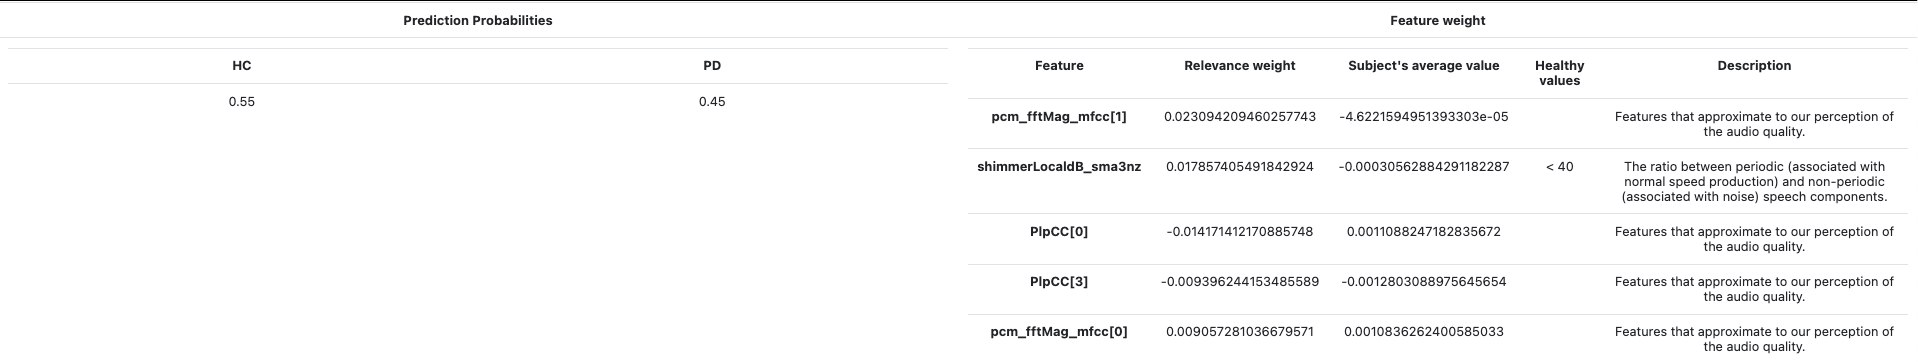
\includegraphics[clip=true, width=\textwidth]{figs/example_explanation.png}
	\end{center}
	\caption{Example of an explanation generated by LIME.}
	\label{explanation}
\end{figure*}

To generate an explanation, the top 5 features with higher contribution to the diagnostic are selected. Figure \ref{explanation} demonstrates an example of an explanation, containing the percentage attributed to each class (\gls{pd} and \gls{hc}), the top features with the highest contribution to the diagnostic, their corresponding weights, normal values and a small description of the feature. This information allows the medical professional to have a more clear understanding of the model's classification. The percentage attributed to each class allows to evaluate the degree of confidence of the model in the decision, whereas the features values can be combined with the normal range of values to check for abnormal parameters. Finally, the feature description connects the mathematical definition of the features with its physical demonstration, thus simplifying the medical professional's ability to interpret the results. 

\subsection{Global Feature Contribution}

\begin{table}
	\centering
	\begin{tabular}{lcccccccc}
		\bfseries feature & \bfseries percentage of subjects & \bfseries contribution (weight)
		\csvreader[head to column names]{csvs/explanation_by_percentage.csv}{}
		{\\\hline\feature & \percentage & \weight}
	\end{tabular}
	\caption{\label{tab:table-name}Top 10 more common features on explanations.}
\end{table}

\begin{table}
	\centering
	\begin{tabular}{lcccccccc}
		\bfseries feature & \bfseries percentage of subjects & \bfseries contribution (weight)
		\csvreader[head to column names]{csvs/explanation_by_weight.csv}{}
		{\\\hline\feature & \percentage & \weight}
	\end{tabular}
	\caption{\label{tab:table-name}Top 10 features ordered by contribution (weight) to explanations.}
	
\end{table}

Tables 5.7 and 5.8 show the top 10 features sorted by their frequency on the complete set of explanations produced in this work and by average contribution to the models' classification, respectively. \\
\gls{plp} and \gls{mfcc} are different mathematical representations of sound that simulate the way humans perceive it. Observing tables 5.7 and 5.8, it is possible to verify that this features represent the majority of the top features with higher contribution to the model's classification of largest number of test subjects. Comparing the \gls{mfcc}s (represented on the table as \textit{pcm\_fftMag\_mfcc[n]}) and \gls{plp}s (represented on the table as \textit{PlpCC[n]}), there are no clear differences between these features. Finally, jitter (represented on the table as \textit{jitterLocal\_sma3nz}) is also on the top features with higher weight contribution. \\
On the other hand, \gls{f0}, shimmer and \gls{hnr} produce significant contributions to few test subjects (8.2\% for F0, 7.4\% for shimmer and 6.5\% for HNR). These features' contributions are inferior to the ones shown on the table (0.0437 for F0, 0.0402 for HNR and 0.0379 for shimmer). A we can observe in figure \ref{weight}. The global contribution (weight) for each feature can be observed in figure \ref{weight}. The weight of the feature with highest global contribution is around 66\% larger the weight from the feature with lowest contribution. However, as there is no significant difference between one feature's value and the following, there is no evident way of splitting the features in two groups and label them as \textit{relevant} and \textit{non-relevant}.

\begin{landscape}
	\begin{figure*}[t]
		\begin{center}
			%\scalebox{1}[-1]{ 
				%\scalebox{-1}[1]{
				    \rotatebox[origin=c]{180}{
						\includegraphics[clip=false,height=0.95\textwidth,width=0.95\textwidth]{figs/feature_by_weight.png}
					}
				%}
			%}
		\end{center}
		\caption{Global contribution (weight) by feature.}
		\label{weight}
	\end{figure*}
\end{landscape}

\begin{landscape}
	\begin{figure*}[t]
		\begin{center}
			%\scalebox{1}[-1]{ 
			%\scalebox{-1}[1]{
			\rotatebox[origin=c]{180}{
				\includegraphics[clip=false,height=0.95\textwidth,width=0.95\textwidth]{figs/feature_by_percentage.png}
			}
			%}
			%}
		\end{center}
		\caption{Percentage of subjects by feature.}
		\label{percentage}
	\end{figure*}
\end{landscape}

